\chapter{Анализ предметной области}

\section{Детерминированный подход}

Детерминированный подход основывается на сравнении характеристик распознаваемого объекта с эталонными признаками. 

В рамках этого подхода используется множество методов, среди которых наиболее известным является метод контурного анализа~\cite{contur_analysis}.

Контурный анализ является совокупностью методов выделения, описания и преобразования контуров изображений и распознавания зрительных образов. Контур целиком определяет форму изображения и содержит всю необходимую информацию для распознавания изображений по их форме. Такой подход позволяет не рассматривать внутренние точки изображения и тем самым значительно сократить объем обрабатываемой информации. Следствием этого является возможность обеспечения работы системы в режиме реального времени.

Основные этапы детерминированного подхода можно разбить на четыре шага:

\begin{enumerate}
    \item разрывы контура в местах, где яркость меняется не слишком быстро;
    \item наличие ложных контуров вследствие шума на изображении;
    \item широкие контурные линии из-за размытости или шума.
\end{enumerate}

Преимуществом данного подхода является то, что для поиска и классификации объектов необходимы только эталонные изображения.

В качестве основного недостатка детерминированного подхода выделяют неустойчивость к шумам на используемых изображениях.

\clearpage

\section{Экспертный подход}

Экспертный подход основан на разделении множества входных объектов по определенным критериям. Одним из основных методов, использующих данный подход, является дерево решений~\cite{solution_tree}. 

Дерево решений представляет собой иерархическую древовидную структуру, в узлах которой содержатся условия, генерируемые в процессе обработки обучающего набора данных. Листья дерева представляют собой классы, по которым производится классификация объектов.

Процесс построения дерева решений включает рекуррентное разбиение обучающего множества на подмножества с применением решающих правил в узлах дерева. Разбиение продолжается до тех пор, пока во всех листьях не окажется конкретный класс, по которому производится классификация. Узел становится листом, когда он содержит объекты одного класса или когда достигается одно из условий остановки, например, максимальная глубина дерева.

Для построения дерева решений обычно применяются жадные алгоритмы, которые выбирают оптимальные решения на каждом шаге алгоритма, но не могут вернуться и изменить их позднее, даже если это было бы оптимальнее для всей системы. На каждом шаге выбирается условие, максимизирующее функцию прироста информации. Для вычисления этой функции используется, например, средняя квадратичная ошибка~\ref{mse}.

\begin{equation}
    \label{mse}
    MSE = \frac{1}{n} \sum_{i=1}^{n} (y_{\text{true}} - y_{\text{pred}_i})^2,
\end{equation}

где:

\begin{itemize}
    \item[---] $ n $ — число элементов в подмножестве;
    \item[---] $ y_{\text{true}} $ — истинное значение атрибута;
    \item[---] $ y_{\text{pred}_i} $ — предсказанное значение атрибута для $ i $-го элемента подмножества.
\end{itemize}

\clearpage

Функция прироста информации может быть выражена зависимостью~\ref{ig}.

\begin{equation}
    \label{ig}
    IG = MSE_{\text{root}} - \left( \frac{n_{\text{left}}}{n} MSE_{\text{left}} - \frac{n_{\text{right}}}{n} MSE_{\text{right}} \right),
\end{equation}

где $ MSE_{\text{root}} $ — ошибка в корневом узле, $ MSE_{\text{left}} $ и $ MSE_{\text{right}} $ — ошибки в левом и правом подмножествах соответственно.

Таким образом, на каждом шаге алгоритм выбирает условие, для которого функция прироста информации будет максимальной. Процесс построения дерева останавливается, когда значение функции ошибки равно нулю или когда в узле остается только один элемент, который считается листом.

\section{Нейронные сети}

Нейронная сеть - компьютерная программа, которая работает по принципу естественной нейронной сети в мозгу. Задача таких искусственных нейронных сетей - выполнять такие когнитивные функции, как решение проблем и машинное обучение. Теоретические основы нейронных сетей были разработаны в 1943 году нейрофизиологом Уорреном Маккалоком из Университета Иллинойса и математиком Уолтером Питтсом из Чикагского университета. В 1954 году Белмонту Фарли и Уэсли Кларку из Массачусетского технологического института удалось запустить первую простую нейронную сеть. Основная привлекательность нейронных сетей - их способность имитировать умение мозга распознавать образы~\cite{neural_network}.

Нейронные сети, хотя и не являются точной моделью человеческого мозга, имеют два важных сходства с ним:

\begin{itemize}
    \item[---] они обучаются, анализируя данные из внешней среды;
    \item[---] их память и обработка информации основаны на связях между искусственными нейронами.
\end{itemize}

Благодаря этим характеристикам, нейронные сети обладают рядом преимуществ перед традиционными алгоритмическими системами. Они способны обрабатывать данные параллельно, работать без детально прописанных инструкций и выявлять глобальные закономерности в данных.

Однако такие особенности создают и определенные ограничения: для обучения требуется значительный объем данных, точность вывода не всегда высока, а процесс обучения может быть крайне ресурсоемким.

Существует несколько подходов к построению нейронных сетей, среди которых можно выделить:

\begin{itemize}
    \item[---] перцептрон;
    \item[---] сверточные нейронные сети;
    \item[---] капсульные нейронные сети.
\end{itemize}

\subsection{Перцептрон}

Впервые словосочетание «искусственная нейронная сеть» употребили в статье «Логическое исчисление идей, относящихся к нервной активности». Но развил и воплотил эти идеи в жизнь американский нейрофизик Фрэнк Розенблатт. В 1958 году он предложил схему устройства, моделирующего человеческое восприятие, и назвал его перцептрон (от англ. perception-восприятие). Функция перцептрона заключалась в том, что он должен был передавать информацию от «глаз», представляющих собой фотоэлементы, в блоки электромеханических ячеек памяти, которые по принципам коннективизма абсолютно случайно соединялись между собой. И уже в 1960 в Корнелльском университете был создана и представлена миру физическая модель перцептрона-компьютер Марк 1, который мог различать некоторые буквы английского алфавита на карточках, подносимых к камерам. Основная особенность нейросетей это способность к самообучению и улучшению, уточнению своей функции~\cite{tlu}. 

\clearpage

Схема элементарного перцептрона представлена на рисунке~\ref{tlu_sheme}.

\begin{figure}[H]
    \centering
    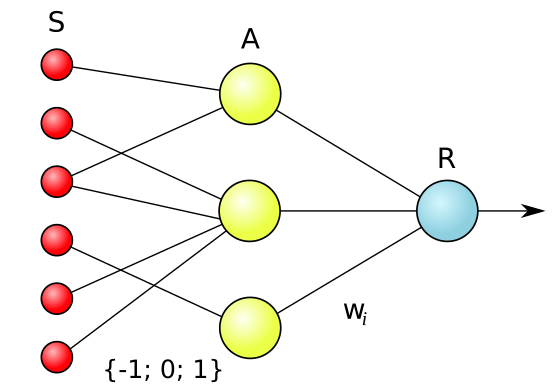
\includegraphics[width=0.6\linewidth]{images/tlu.png}
    \caption{Схема элементарного перцептрона}
    \label{tlu_sheme}
\end{figure}

Элементарный перцептрон состоит из элементов трех типов: $S$-элементов, $A$-элементов и одного $R$-элемента. 

$S$-элементы — это слой сенсоров или рецепторов. Каждый рецептор может находиться в одном из двух состояний — покоя или возбуждения, и только в последнем случае он передает единичный сигнал в следующий слой, ассоциативным элементам.

$A$-элементы называются ассоциативными, потому что каждому такому элементу, как правило, соответствует целый набор $S$-элементов. $A$-элемент активизируется, как только количество сигналов от $S$-элементов на его входе превысило некоторую величину $\theta$

Сигналы от возбудившихся $A$-элементов, в свою очередь, передаются в сумматор $R$, причем сигнал от $i$-го ассоциативного элемента передается с коэффициентом $w_i$. Этот коэффициент называется весом $A$—$R$ связи.

$R$-элемент подсчитывает сумму значений входных сигналов, помноженных на веса. $R$-элемент, а вместе с ним и элементарный перцептрон, выдает $1$, если линейная форма превышает порог $\theta$, иначе на выходе будет $-1$. Математически функцию, реализуемую $R$-элементом, можно записать в виде формулы~\ref{tlu_formular}.

\begin{equation}
    \label{tlu_formular}
    f(x) = sign(\sum_{i=1}^nw_ix_i-\theta)
\end{equation}

\subsection{Сверточные нейронные сети}

Сверточная нейронная сеть (CNN) очень похожа на зрительную кору головного мозга. На зрительной коре имеются небольшие участки клеток нейронов, которые связаны с определенными местами зрительного поля. За это открытие Дэвид Хьюбел и Торстен Визель удостоились Нобелевской премии по медицине 1981 года. Хьюбел и Визель в 1962 году провели эксперимент, в котором показали, что отдельные клетки нейронов откликались исключительно при наблюдении границ конкретной ориентации~\cite{cnn}.

Если рассматривать CNN более подробно, то она состоит из серии слоев. Берется изображение, пропускается через чередование сверточных, нелинейных слоев, и с помощью полносвязного слоя порождается вывод. В качестве вывода может выступать класс или вероятность класса, которое лучше всего описывает изображение. 

Сверточный слой – это слой, на которым при помощи операции математической свертки заданное количество ядер или окон фильтров в виде матриц также заданного размера проходят построчно по входящей матрице, формируя новую матрицу. Ядро фильтра – матрица весов, которая путем свертки извлекает признаки из пришедших данных. Весовые коэффициенты ядра свертки устанавливаются в процессе обучения и изначально не определены. Фильтр – это объединение нескольких ядер.

Количество фильтров на сверточном слое задается на основе исходной задачи и требований к ее решению: чем фильтров больше, тем выше качество распознавание и ниже быстродействие~\cite{cnn_more}.

Схема cверточной нейронной сети представлена на рисунке~\ref{cnn_sheme}.

\begin{figure}[H]
    \centering
    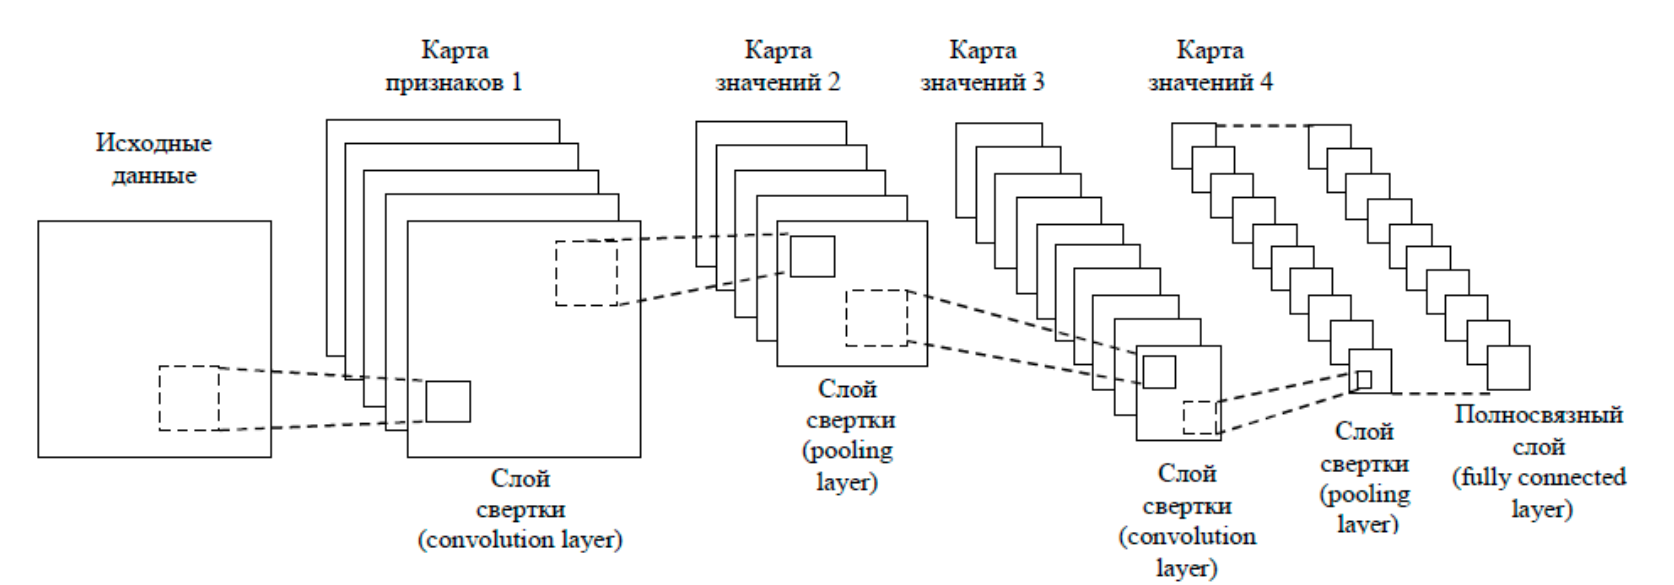
\includegraphics[width=0.8\linewidth]{images/cnn.png}
    \caption{Схема cверточной нейронной сети}
    \label{cnn_sheme}
\end{figure}

\subsection{Капсульные нейронные сети}

Капсульные нейронные сети содержат так называемый капсульный слой. Капсула — это модифицированный искусственный нейрон, расширенный от скалярной к векторной форме, что позволяет ей хранить больше информации об объекте. На выходе капсулы формируется вектор, способный описывать состояние объекта, например, его позу. Длина вектора определяет вероятность обнаружения объекта, а его направление указывает на состояние объекта~\cite{capsnet}.

Функция активации в капсулах задается следующим образом:
$$
v_j = \frac{{||s_j||^2}}{{1 + ||s_j||^2}} \cdot \frac{{s_j}}{{||s_j||}},
$$
где $v_j$ — выходной вектор капсулы $j$, $s_j$ — входной вектор. Правая часть этого выражения делает вектор $s_j$ единичным, а левая выполняет масштабирование так, что длина $v_j$ приближается к 1 для больших значений $s_j$ и к 0 для малых значений.

Для всех капсул, кроме капсул первого слоя, вход $s_j$ является взвешенной суммой по всем векторам предсказаний $u_{ji}$ от капсул предыдущего слоя, которые получаются умножением выхода $u_i$ капсулы нижележащего слоя на весовую матрицу $W_{ij}$. Таким образом, вход в капсулу $j$ определяется выражением:
$$
s_j = \sum_i c_{ij} u_{ji},
$$
где $c_{ij}$ — коэффициент связи между капсулами $i$ и $j$, который рассчитывается по формуле:
$$
c_{ij} = \frac{e^{b_{ij}}}{\sum_k b_{ik}},
$$
где $b_{ij}$ — вероятность того, что капсула $i$ связана с капсулой $j$. Эти вероятности обновляются итеративно, измеряя степень соответствия между текущим выходом $\mathbf{v}_j$ капсулы $j$ и предсказанием $\mathbf{u}_{ji}$ капсулы $i$. Соответствие рассчитывается как скалярное произведение $\mathbf{v}_j$ и $\mathbf{u}_{ji}$.

\clearpage

Схема капсульной нейронный сети представленна на рисунке~\ref{capsnet_sheme}.

\begin{figure}[H]
    \centering
    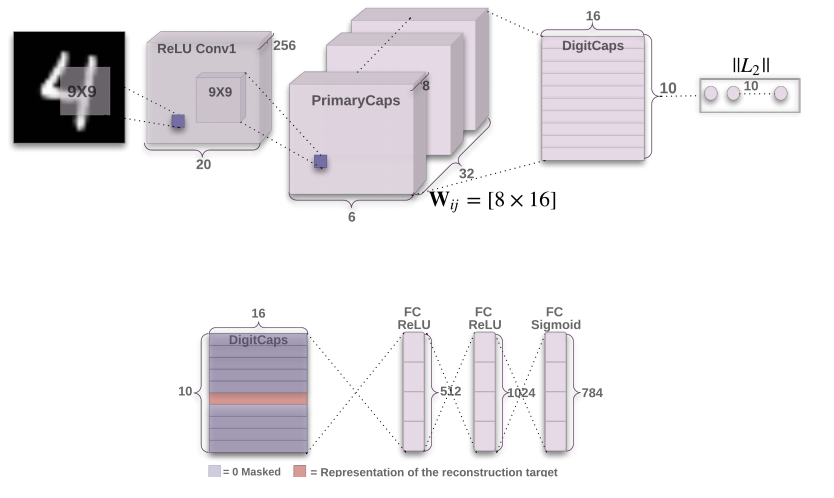
\includegraphics[width=0.8\linewidth]{images/capsnet.png}
    \caption{Схема капсульной нейронной сети}
    \label{capsnet_sheme}
\end{figure}

\chapter{Анализ существующих решений}

Для решения задачи классификации объектов на изображениях наиболее рационально использовать нейронные сети. Детерминированные методы здесь не подходят, поскольку они неустойчивы к шуму в данных, а метод дерева решений оказывается неприменим из-за отсутствия четких критериев для классификации на этапе построения дерева. Следующим этапом работы станет выбор оптимальной архитектуры нейронной сети.

Полносвязные сети, такие как перцептрон, имеют ограниченное применение в задачах с большим числом входных данных, поскольку сложность их вычислений растет экспоненциально по мере увеличения размеров входных векторов.

Капсульные нейронные сети, хотя и позволяют учитывать пространственное положение объектов, не являются подходящим выбором для данной задачи. Их основное преимущество — выделение иерархических структур в данных — требует значительных вычислительных ресурсов, что делает их менее эффективными для анализа больших изображений. Кроме того, капсульные сети уступают сверточным по устойчивости к шуму, что может отрицательно сказаться на точности классификации~\cite{capsnet_minus}.

Для поиска и классификации объектов на изображениях существует множество модификаций сверточных нейронных сетей~\cite{cnn_types}, среди которых наиболее популярными являются:

\begin{itemize}
    \item[---] семейство сетей YOLO;
    \item[---] Single Shot Detection;
    \item[---] R-CNN и его модификации.
\end{itemize}

\clearpage

\section{Семейство нейронных сетей YOLO}

YOLO (You Only Look Once) — это алгоритм, который выполняет обнаружение объектов и определение их местоположения на изображении за один проход~\cite{yolo}. YOLO применяет нейронные сети для идентификации объектов в режиме реального времени, и его развитие прошло через несколько версий: от первой YOLOv1 до последующих версий YOLOv2, YOLOv3 и так далее.

Архитектура YOLO построена на основе сверточной нейронной сети (CNN) для выполнения задачи обнаружения объектов. YOLO анализирует изображение целиком, предсказывая ограничивающие рамки и вероятности классов для обнаруженных объектов.Это единая сверточная нейронная сеть, которая одновременно выполняет обнаружение нескольких объектов, определяет их границы и оценивает вероятность принадлежности каждого к определенному классу.

YOLO работает в несколько этапов.
\begin{enumerate}
    \item Масштабирование изображения до фиксированного размера, например, 416x416, для единообразной обработки.
    \item Разделение изображения на сетку $N \times N$ (например, 13x13) ячеек для локализации объектов.
    \item Прогон изображения через сверточную нейронную сеть (CNN), которая извлекает важные признаки для последующей обработки.
    \item Прогнозирование нескольких ограничивающих рамок для каждой ячейки сетки, включая координаты, размеры и вероятности классов.
    \item Фильтрация рамок по вероятности — рамки с низкой уверенностью отбрасываются.
    \item Применение подавления неперекрывающихся рамок (NMS) для устранения наложений и выбора лучших рамок.
    \item Возврат окончательных рамок и меток классов для обнаруженных объектов.
\end{enumerate}

Схема YOLO представлена на рисунке~\ref{yolo_sheme}.

\begin{figure}[H]
    \centering
    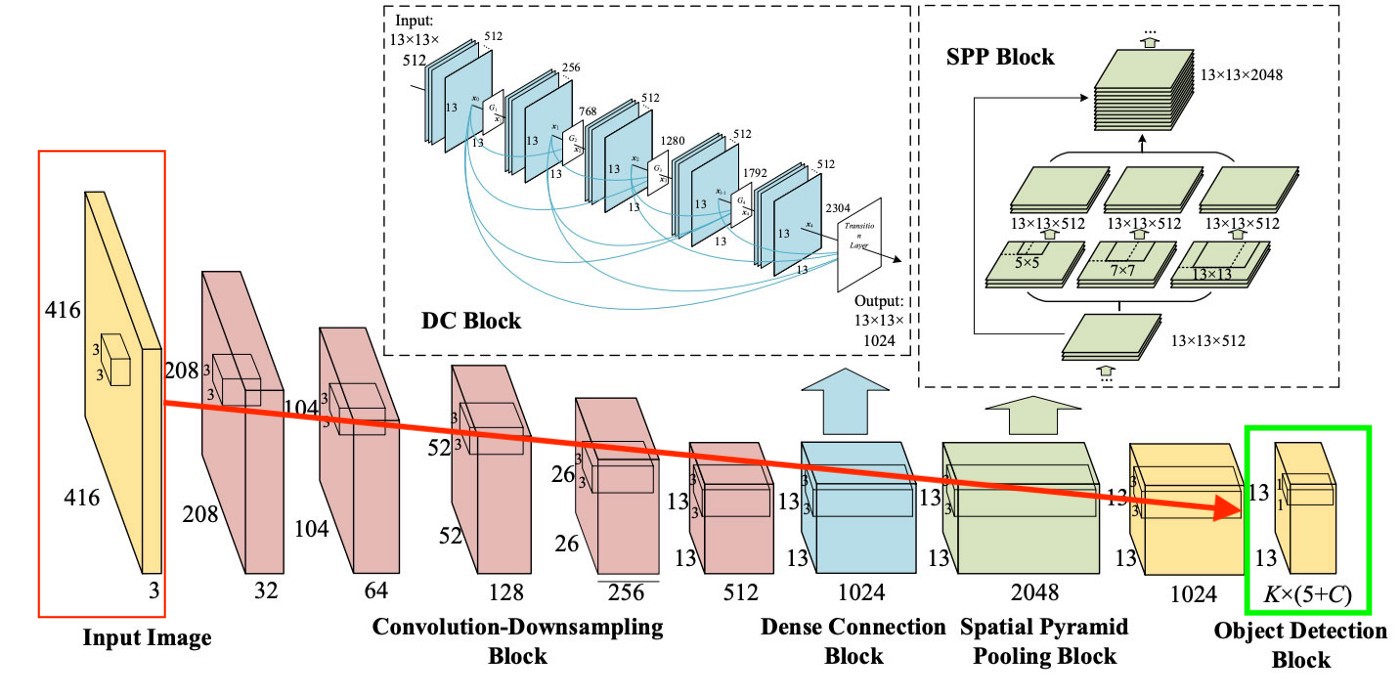
\includegraphics[width=0.8\linewidth]{images/yolo.png}
    \caption{Схема YOLO}
    \label{yolo_sheme}
\end{figure}

\section{Single Shot Detection}

Single Shot Detection (SSD) использует в своей основе предварительно обученные модели, такие как VGG или ResNet, которые были разработаны для задач классификации на больших наборах данных. На базовую сеть накладываются дополнительные слои, включающие сверточные и пулинговые операции, что позволяет системе выявлять объекты различных размеров~\cite{ssd}.

Главное преимущество SSD заключается в её высокой скорости обработки: благодаря тому, что вся работа выполняется одной сетью, она подходит для задач, требующих анализа изображений в реальном времени, таких как системы видеонаблюдения или автопилоты.  

Метод SSD эффективно применяет предварительно обученную базовую сеть, что даёт возможность использовать крупные размеченные датасеты, изначально созданные для задач классификации. Однако этот подход имеет свои недостатки. Одной из ключевых проблем является чувствительность к размерам объектов: если их масштаб существенно отличается от объектов, представленных в обучающем наборе, точность обнаружения может снижаться. Это связано с тем, что дополнительные слои сети оптимизированы для обработки объектов лишь в определённых диапазонах размеров.

Схема SSD представлена на рисунке~\ref{ssd_sheme}.

\begin{figure}[H]
    \centering
    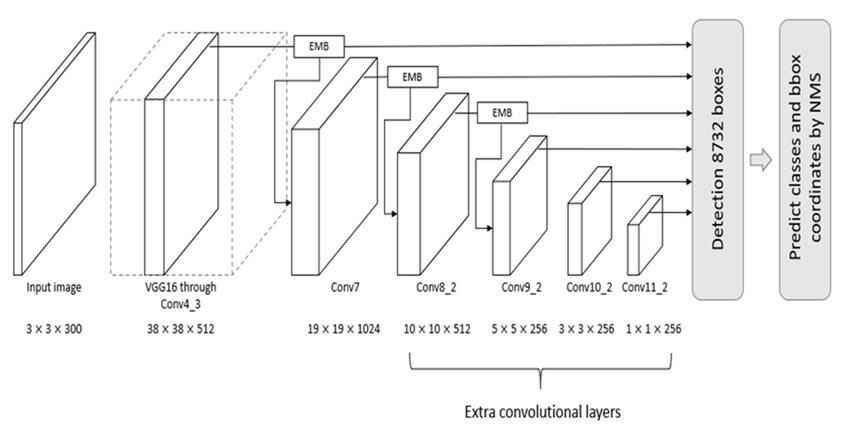
\includegraphics[width=0.8\linewidth]{images/ssd.png}
    \caption{Схема SSD}
    \label{ssd_sheme}
\end{figure}

\section{R-CNN}

R-CNN (Regions with Convolutional Neural Networks) — это метод обнаружения объектов, разработаный командой из UC Berkley, который работает, выделяя потенциальные области, где могут находиться объекты, и применяя сверточные нейронные сети к этим областям для классификации и локализации объектов~\cite{r-cnn}. Процесс можно разделить на несколько основных шагов.

\begin{enumerate}
    \item R-CNN сначала применяет алгоритм, такой как Selective Search, чтобы сгенерировать около 2000 регионов-кандидатов.
    \item Каждая из этих областей изменяется под фиксированный размер, чтобы затем передать в нейронную сеть для обработки.
    \item Каждый выделенный регион проходит через сверточную нейронную сеть. На этом этапе R-CNN определяет, какой объект находится в регионе, и создает ограничивающую рамку для точного выделения его позиции.
    \item Для повышения точности рамки дополнительно корректируются с использованием регрессионной модели, чтобы максимально соответствовать границам объекта.
    \item На основе предсказанных классов и рамок, R-CNN отфильтровывает регионы, чтобы получить окончательные результаты.
\end{enumerate}

Схема R-CNN представлена на рисунке~\ref{r-cnn_sheme}.

\begin{figure}[H]
    \centering
    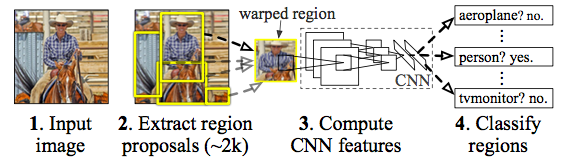
\includegraphics[width=0.8\linewidth]{images/r-cnn.png}
    \caption{Схема R-CNN}
    \label{r-cnn_sheme}
\end{figure}

Метод R-CNN обеспечивает хорошее качество обнаружения, но имеет ряд недостатков:

\begin{itemize}
    \item[---] Поскольку R-CNN использует разные модели для каждого этапа, каждая из них обучается отдельно, что может приводить к несовместимым результатам;
    \item[---] R-CNN обрабатывает каждый регион-кандидат отдельно, что требует значительных вычислительных ресурсов и времени;
    \item[---] R-CNN требует нескольких этапов обучения: сначала обучается модель для выделения регионов, затем модель для классификации, и дополнительно — для регрессии ограничивающих рамок.
\end{itemize}

\section{Fast R-CNN}

Fast R-CNN была разработана для преодоления недостатков медлительности и сложности обучения, характерных для R-CNN~\cite{fast_r-cnn}. В отличие от R-CNN, где для каждого региона-кандидата выполнялось отдельное прохождение сети, в Fast R-CNN все изображение пропускается через сверточные слои один раз. Это позволяет эффективно извлекать признаки для всего изображения сразу. После извлечения признаков для всего изображения, Fast R-CNN использует RoI-пулинг, чтобы выделить соответствующие регионы-кандидаты (регион интереса, RoI). RoI-пулинг преобразует размер этих регионов в фиксированный, что позволяет обрабатывать их в одном этапе. Каждый регион-кандидат классифицируется в один из классов объектов, а также предсказывается точная позиция ограничивающей рамки для каждого объекта. Эти два этапа выполняются параллельно, что ускоряет обработку.

Схема Fast R-CNN представлена на рисунке~\ref{fast_r-cnn_sheme}.

\begin{figure}[H]
    \centering
    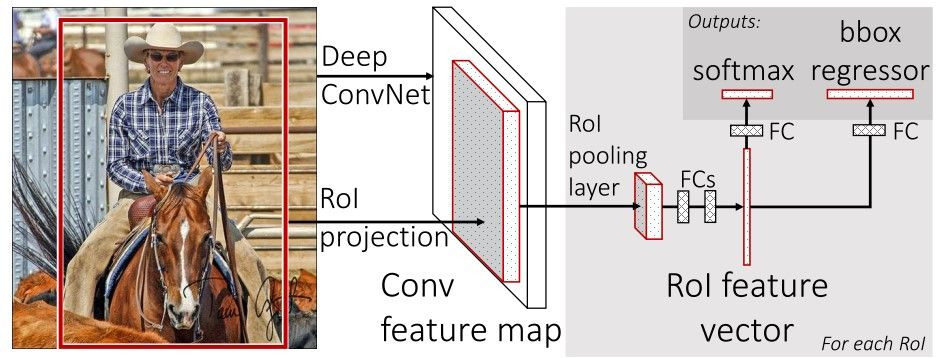
\includegraphics[width=0.8\linewidth]{images/fast_r-cnn.png}
    \caption{Схема Fast R-CNN}
    \label{fast_r-cnn_sheme}
\end{figure}

Основная причина, по которой Fast R-CNN работает быстрее, чем R-CNN, заключается в том, что сверточная операция выполняется только один раз для каждого изображения, а не для 2000 регионов-кандидатов. Это позволяет сразу получить карту признаков, из которой выделяются необходимые регионы.

Fast R-CNN значительно ускоряет процесс обучения и тестирования по сравнению с R-CNN. Тем не менее, генерация регионов-кандидатов продолжает быть основным ограничивающим фактором, который сдерживает производительность алгоритма.

\section{Faster R-CNN}

Оба упомянутых алгоритма, R-CNN и Fast R-CNN, используют метод выборочного поиска для формирования регионов-кандидатов, что является медленным и требовательным к ресурсам процессом, ограничивающим общую производительность сети. Чтобы решить эту проблему, Шаочин Рен и коллеги предложили алгоритм обнаружения объектов, который исключает выборочный поиск, позволяя сети самостоятельно генерировать регионные предложения~\cite{faster_r-cnn}.

В алгоритме Faster R-CNN, как и в Fast R-CNN, изображение сначала пропускается через сверточную сеть для создания карты признаков. Однако, вместо применения медленного выборочного поиска для выделения регионов-кандидатов, Faster R-CNN использует дополнительную сеть — Region Proposal Network (RPN), которая эффективно предсказывает области, вероятно содержащие объекты. Далее, с помощью слоя Region of Interest (RoI) Pooling, эти регионные предложения адаптируются для классификации объектов и уточнения координат ограничивающих рамок. Этот подход делает процесс выделения областей намного более быстрым и точным, что позволяет обрабатывать изображения в реальном времени и обеспечивает высокую эффективность модели в задачах обнаружения объектов.

Схема Faster R-CNN представлена на рисунке~\ref{faster_r-cnn_sheme}.

\begin{figure}[H]
    \centering
    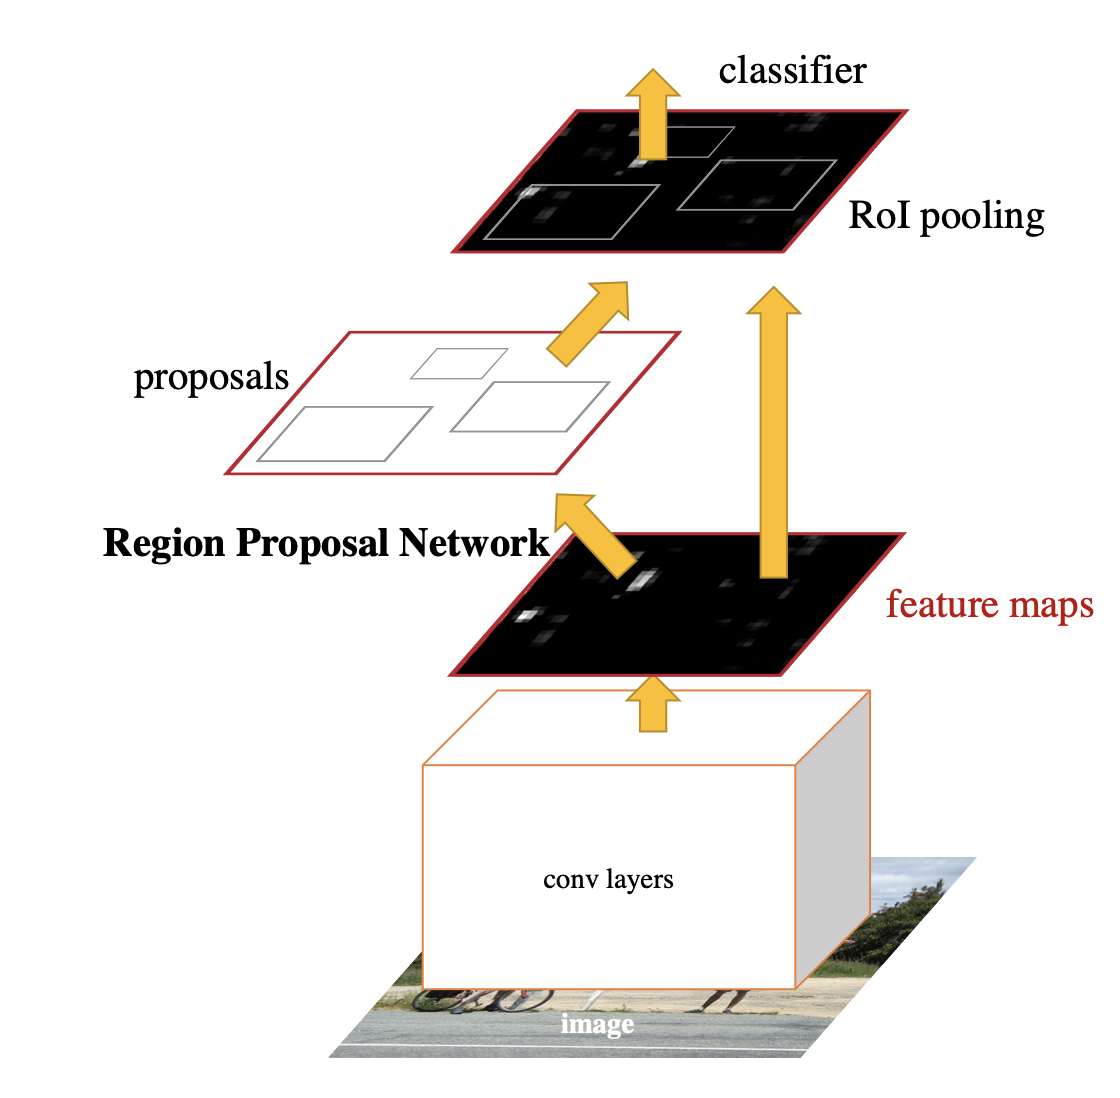
\includegraphics[width=0.8\linewidth]{images/faster_r-cnn.png}
    \caption{Схема Fast R-CNN}
    \label{faster_r-cnn_sheme}
\end{figure}

Сравнение скорости R-CNN, Fast R-CNN и Faster R-CNN представлено на рисунке~\ref{r-cnn_comp}~\cite{r-cnn_comp}.

\begin{figure}[H]
    \centering
    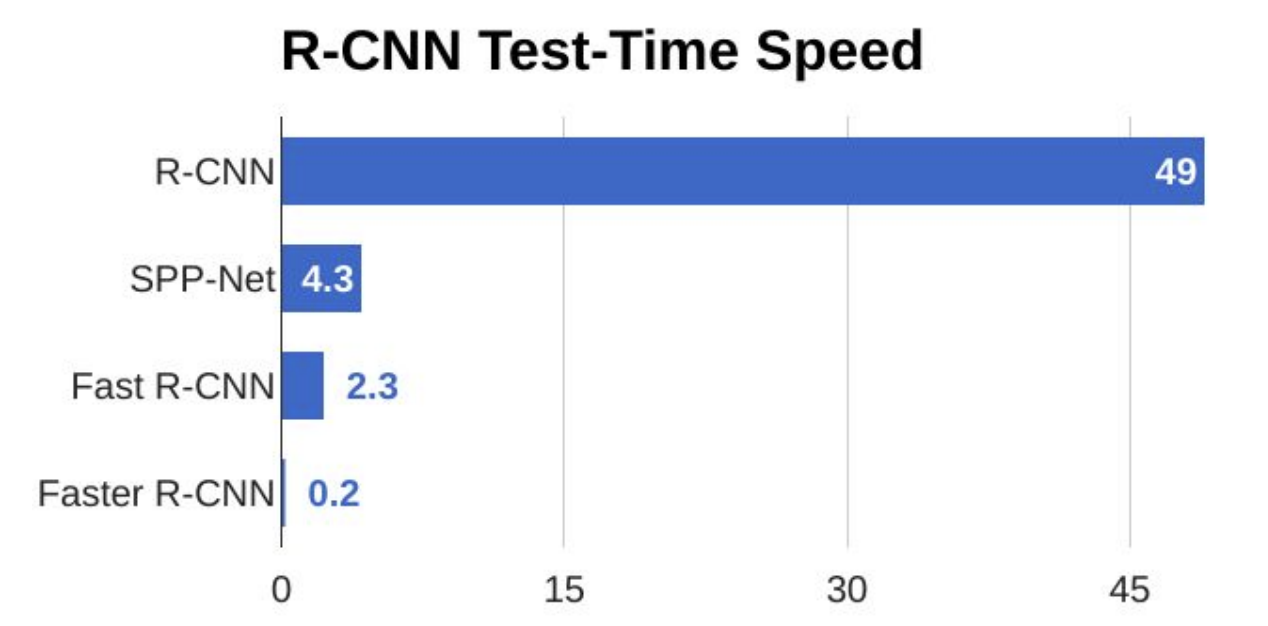
\includegraphics[width=0.8\linewidth]{images/r-cnn_comp.png}
    \caption{Сравнение скорости R-CNN, Fast R-CNN и Faster R-CNN}
    \label{r-cnn_comp}
\end{figure}

Сравнение средней точности и скорости обработки изображений на разных наборах данных R-CNN, Fast R-CNN, Faster R-CNN представлено на таблице~\ref{tbl:r-cnn_mes}~\cite{all_comp_with_yolov7}.

\begin{table}[H]
    \centering
    \begin{threeparttable}
    \caption{Сравнение R-CNN, Fast R-CNN и Faster R-CNN}
    \captionsetup{justification=raggedright, singlelinecheck=false}
    \label{tbl:r-cnn_mes}
    \begin{tabular}{|>{\centering\arraybackslash}m{4cm}|>{\centering\arraybackslash}m{4cm}|>{\centering\arraybackslash}m{4cm}|>{\centering\arraybackslash}m{3cm}|}
        \hline
        \textbf{Модель} & \textbf{Набор данных} & \textbf{Средняя точность (\%)} & \textbf{FPS} \\ \hline
        RCNN & ILSVRC2013 & 31.4 & 0.077 \\ \hline
        RCNN & VOC 2010 & 53.7 & 0.077 \\ \hline
        Fast R-CNN & VOC 2007 & 70 & 3.33 \\ \hline
        Fast R-CNN & VOC 2010 & 68.8 & 3.33 \\ \hline
        Fast R-CNN & VOC 2012 & 68.4 & 3.33 \\ \hline
        Faster R-CNN & VOC 2007 & 78.8 & 5 \\ \hline
        Faster R-CNN & VOC 2012 & 75.9 & 5 \\ \hline
        Faster R-CNN & COCO & 42.1 & 5 \\ \hline
    \end{tabular}
    \end{threeparttable}
\end{table}

На основе таблицы~\ref{tbl:r-cnn_mes} и рисунка~\ref{r-cnn_comp} можно сделать вывод что Faster R-CNN быстрее и точнее своих прдшественников. Исходя из этого дальше будет рассматриваться только Faster R-CNN.

\section{Сравнение решений}

Рассмотренные выше решения были протестированы на скорость и точность работы на наборе данных COCO~\cite{all_comp_with_yolov7}. 

Результаты сравнения существующих решений представлены в таблице~\ref{tbl:mes}.

\begin{table}[H]
    \centering
    \begin{threeparttable}
    \caption{Сравнение существующих решений}
    \captionsetup{justification=raggedright, singlelinecheck=false}
    \label{tbl:mes}
    \begin{tabular}{|>{\centering\arraybackslash}m{30mm}|>{\centering\arraybackslash}m{40mm}|>{\centering\arraybackslash}m{40mm}|>{\centering\arraybackslash}m{40mm}|}
        \hline
          & \textbf{Faster R-CNN} & \textbf{SSD} & \textbf{YOLOv7} \\ \hline
        Скорость (FPS) & 5 & 19 & 161 \\ \hline
        Средняя точность (\%) & 42.1 &  48.5 & 69.7 \\ \hline
        Сложность обучения & Средняя & Средняя & Низкая \\ \hline
        Устойчивость к масштабам & + & + & + \\ \hline
    \end{tabular}
    \end{threeparttable}
\end{table}

Из таблицы~\ref{tbl:mes} можно сделать вывод, что YOLOv7 точнее и быстрее чем Faster R-CNN и SSD, а также легче в обучении.